\section{Chords}

\subsection{Building chords} \label{sec:building-chords-chords-scales}
In the previous sections we have learned about the major and minor scales. This information can be used to finally start to learn about chords.

\textbf{A major or minor chord is constructed by playing the 1st, 3rd and 5th note of a scale at the same time. That's it.}

As seen in \autoref{tab:guitar_major_chord_buildup} and \autoref{tab:guitar_minor_chord_buildup}, in both major and minor scales the 1st, 3rd, and 5th scale indexes (also called scale degrees) are used. The green notes are the root notes. These determine the main name of the chord. The orange ones are the rest of the notes in the chord.

\begin{table}[h]
	\begin{minipage}{0.45\textwidth}
		\centering
		\begin{NiceTabular}{*{16}{P{0.05mm}}}
			\Block{}{} & \Block{1-2}{\large{W}} & & \Block{1-2}{\large{W}} & & \Block{1-2}{\large{H}} & & \Block{1-2}{\large{W}} & & \Block{1-2}{\large{W}} & & \Block{1-2}{\large{W}} & & \Block{1-2}{\large{H}} & & \Block{}{} \\
			\Block[fill=ColorRootNote]{1-2}{1} & & \Block{1-2}{2} & & \Block[fill=ColorOtherNote]{1-2}{3} & & \Block{1-2}{4} & & \Block[fill=ColorOtherNote]{1-2}{5} & & \Block{1-2}{6} & & \Block{1-2}{7} & & \Block{1-2}{8} & 
		\end{NiceTabular}
		\caption{Building up a major chord}
		\label{tab:guitar_major_chord_buildup}
	\end{minipage}
	\hfill
	\begin{minipage}{0.45\textwidth}
		\centering
		\begin{NiceTabular}{*{16}{P{0.05mm}}}
			\Block{}{} & \Block{1-2}{\large{W}} & & \Block{1-2}{\large{H}} & & \Block{1-2}{\large{W}} & & \Block{1-2}{\large{W}} & & \Block{1-2}{\large{H}} & & \Block{1-2}{\large{W}} & & \Block{1-2}{\large{W}} & & \Block{}{} \\
			\Block[fill=ColorRootNote]{1-2}{1} & & \Block{1-2}{2} & & \Block[fill=ColorOtherNote]{1-2}{3$\flat$} & & \Block{1-2}{4} & & \Block[fill=ColorOtherNote]{1-2}{5} & & \Block{1-2}{6$\flat$} & & \Block{1-2}{7$\flat$} & & \Block{1-2}{8} &
		\end{NiceTabular}
		\caption{Building up a minor chord}
		\label{tab:guitar_minor_chord_buildup}
	\end{minipage}
\end{table}

\autoref{tab:guitar_major_chords_from_scales} and \autoref{tab:guitar_minor_chords_from_scales} show the construction of other chords. The order of the chords in the major and minor tables are the same. This way you can compare them. These notes are also seen in the chord charts in \autoref{fig:guitar_major_minor_chords}.

Note how the 1st and 5th note in both major and minor chords are the same. Only the 3rd note is always a half step lower in the minor chord compared to the major chord.

\begin{table}[h]
	\begin{minipage}{0.45\textwidth}
				\centering
		\begin{NiceTabular}{*{16}{P{0.05mm}}}
			\Block{}{} & \Block{1-2}{\large{W}} & & \Block{1-2}{\large{W}} & & \Block{1-2}{\large{H}} & & \Block{1-2}{\large{W}} & & \Block{1-2}{\large{W}} & & \Block{1-2}{\large{W}} & &  \Block{1-2}{\large{H}} & &  \Block{}{} \\
			\Block{1-2}{1} & & \Block{1-2}{2} & & \Block{1-2}{3} & & \Block{1-2}{4} & & \Block{1-2}{5} & & \Block{1-2}{6} & & \Block{1-2}{7} & & \Block{1-2}{8} \\
			\Block[fill=ColorRootNote]{1-2}{A} & & \Block{1-2}{B} & & \Block[fill=ColorOtherNote]{1-2}{C\sharp} & & \Block{1-2}{D} & & \Block[fill=ColorOtherNote]{1-2}{E} & & \Block{1-2}{F\sharp} & & \Block{1-2}{G\sharp} & & \Block{1-2}{A} \\
			\Block[fill=ColorRootNote]{1-2}{B} & & \Block{1-2}{C\sharp} & & \Block[fill=ColorOtherNote]{1-2}{D\sharp} & & \Block{1-2}{E} & & \Block[fill=ColorOtherNote]{1-2}{F\sharp} & & \Block{1-2}{G\sharp} & & \Block{1-2}{A\sharp} & & \Block{1-2}{B} \\
			\Block[fill=ColorRootNote]{1-2}{C} & & \Block{1-2}{D} & & \Block[fill=ColorOtherNote]{1-2}{E} & & \Block{1-2}{F} & & \Block[fill=ColorOtherNote]{1-2}{G} & & \Block{1-2}{A} & & \Block{1-2}{B} & & \Block{1-2}{C} \\
			\Block[fill=ColorRootNote]{1-2}{D} & & \Block{1-2}{E} & & \Block[fill=ColorOtherNote]{1-2}{F\sharp} & & \Block{1-2}{G} & & \Block[fill=ColorOtherNote]{1-2}{A} & & \Block{1-2}{B} & & \Block{1-2}{C\sharp} & & \Block{1-2}{D} \\
			\Block[fill=ColorRootNote]{1-2}{E} & & \Block{1-2}{F\sharp} & & \Block[fill=ColorOtherNote]{1-2}{G\sharp} & & \Block{1-2}{A} & & \Block[fill=ColorOtherNote]{1-2}{B} & & \Block{1-2}{C\sharp} & & \Block{1-2}{D\sharp} & & \Block{1-2}{E} \\
			\Block[fill=ColorRootNote]{1-2}{F} & & \Block{1-2}{G} & & \Block[fill=ColorOtherNote]{1-2}{A} & & \Block{1-2}{B\flat} & & \Block[fill=ColorOtherNote]{1-2}{C} & & \Block{1-2}{D} & & \Block{1-2}{E} & & \Block{1-2}{F} \\
			\Block[fill=ColorRootNote]{1-2}{G} & & \Block{1-2}{A} & & \Block[fill=ColorOtherNote]{1-2}{B} & & \Block{1-2}{C} & & \Block[fill=ColorOtherNote]{1-2}{D} & & \Block{1-2}{E} & & \Block{1-2}{F\sharp} & & \Block{1-2}{G} \\
		\end{NiceTabular}
		\caption{Major chords from the major scale}
		\label{tab:guitar_major_chords_from_scales}
	\end{minipage}
	\hfill
	\begin{minipage}{0.45\textwidth}
		\centering
		\begin{NiceTabular}{*{16}{P{0.05mm}}}
			\Block{}{} & \Block{1-2}{\large{W}} & & \Block{1-2}{\large{H}} & & \Block{1-2}{\large{W}} & & \Block{1-2}{\large{W}} & & \Block{1-2}{\large{H}} & & \Block{1-2}{\large{W}} & & \Block{1-2}{\large{W}} & & \Block{}{} \\
			\Block{1-2}{1} & & \Block{1-2}{2} & & \Block{1-2}{3$\flat$} & & \Block{1-2}{4} & & \Block{1-2}{5} & & \Block{1-2}{6$\flat$} & & \Block{1-2}{7$\flat$} & & \Block{1-2}{8} \\
			\Block[fill=ColorRootNote]{1-2}{ A} & & \Block{1-2}{B} & & \Block[fill=ColorOtherNote]{1-2}{ C} & & \Block{1-2}{D} & & \Block[fill=ColorOtherNote]{1-2}{ E} & & \Block{1-2}{F} & & \Block{1-2}{G} & & \Block{1-2}{A} \\
			\Block[fill=ColorRootNote]{1-2}{ B} & & \Block{1-2}{C\sharp} & & \Block[fill=ColorOtherNote]{1-2}{ D} & & \Block{1-2}{E} & & \Block[fill=ColorOtherNote]{1-2}{ F\sharp} & & \Block{1-2}{G} & & \Block{1-2}{A} & & \Block{1-2}{B} \\
			\Block[fill=ColorRootNote]{1-2}{ C} & & \Block{1-2}{D} & & \Block[fill=ColorOtherNote]{1-2}{ E\flat} & & \Block{1-2}{F} & & \Block[fill=ColorOtherNote]{1-2}{ G} & & \Block{1-2}{A\flat} & & \Block{1-2}{B\flat} & & \Block{1-2}{C} \\
			\Block[fill=ColorRootNote]{1-2}{ D} & & \Block{1-2}{E} & & \Block[fill=ColorOtherNote]{1-2}{ F} & & \Block{1-2}{G} & & \Block[fill=ColorOtherNote]{1-2}{ A} & & \Block{1-2}{B\flat} & & \Block{1-2}{C} & & \Block{1-2}{D} \\
			\Block[fill=ColorRootNote]{1-2}{ E} & & \Block{1-2}{F\sharp} & & \Block[fill=ColorOtherNote]{1-2}{ G} & & \Block{1-2}{A} & & \Block[fill=ColorOtherNote]{1-2}{ B} & & \Block{1-2}{C} & & \Block{1-2}{D} & & \Block{1-2}{E} \\
			\Block[fill=ColorRootNote]{1-2}{ F} & & \Block{1-2}{G} & & \Block[fill=ColorOtherNote]{1-2}{ A\flat} & & \Block{1-2}{B\flat} & & \Block[fill=ColorOtherNote]{1-2}{ C} & & \Block{1-2}{D\flat} & & \Block{1-2}{E\flat} & & \Block{1-2}{F} \\
			\Block[fill=ColorRootNote]{1-2}{ G} & & \Block{1-2}{A} & & \Block[fill=ColorOtherNote]{1-2}{ B\flat} & & \Block{1-2}{C} & & \Block[fill=ColorOtherNote]{1-2}{ D} & & \Block{1-2}{E\flat} & & \Block{1-2}{F} & & \Block{1-2}{G} \\
		\end{NiceTabular}
		\caption{Minor chords from the minor scale}
		\label{tab:guitar_minor_chords_from_scales}
	\end{minipage}
\end{table}

\newpage

\subsection{Open and barre chords}

When a chords is played that contains open strings, it is called an "open chord" (e.g. \autoref{fig:guitar-open-c-chord-hand-position}). When a chord is played without open strings, it is called a "Closed chord" or "barre chord" (e.g. \autoref{fig:guitar-barre-f-chord-hand-position}). Note that a barre chord is a type of closed chord.

\begin{figure}[h]
	\begin{subfigure}[b]{0.45\textwidth}
		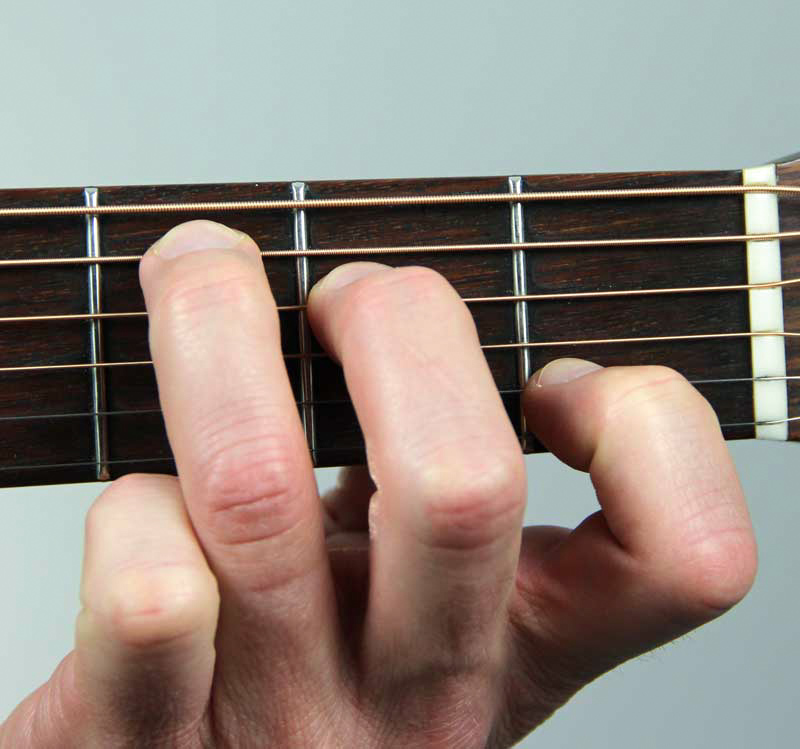
\includegraphics[width=\textwidth]{../../Images/open-c-chord.jpg}
		\caption{Open C chord \cite{OpenCChordHand}}
		\label{fig:guitar-open-c-chord-hand-position}
	\end{subfigure}
	\hfill
	\begin{subfigure}[b]{0.45\textwidth}
		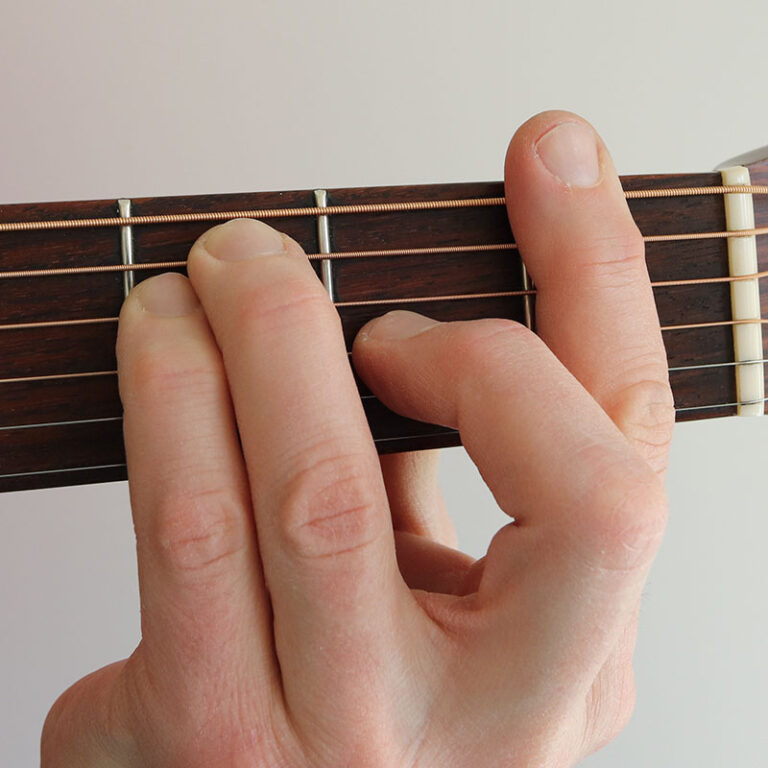
\includegraphics[width=\textwidth]{../../Images/F-major-barre-photo-768x768.jpg}
		\caption{Barre F chord \cite{BarreFChordHand}}
		\label{fig:guitar-barre-f-chord-hand-position}
	\end{subfigure}
	\caption{}
\end{figure}


The nice thing about closed/barre chords is that you can move them up and down the neck. At that point the closed/barre chord becomes more of a shape than a chord per se. Depending on what the root note is at a certain position, the barre chord will get a different name. We will see this later in the \textbf{CAGED system}.

On the next page in \autoref{fig:guitar_major_minor_chords} you will see all the major and minor chords listed. The chord \textbf{C} is a major chord and the chord \textbf{Cm} is a minor chords. The same holds for the other chords. Below each chords there are the 1st, 3rd and 5th notes from the respective scale that make up the chord (see \autoref{tab:guitar_major_chords_from_scales} and \autoref{tab:guitar_minor_chords_from_scales}).

The green dots indicate the root note. This note determines the main name of the chord.

A couple things to note:

\begin{itemize}
	\item The root and the 5th note of a scale are same for both the major and minor variant.
	\item The 3rd note of minor chord is always a half step / 1 semitone lower than it is in the major chord.
\end{itemize}

\newpage

% Billie eilish Therefore I am: Dm A - i V
% Robin Thicke Blurred Lines: G D - I V
% Arctic Monkeys - 505: Dm Em - i ii


\begin{figure}[h]
	\centering
	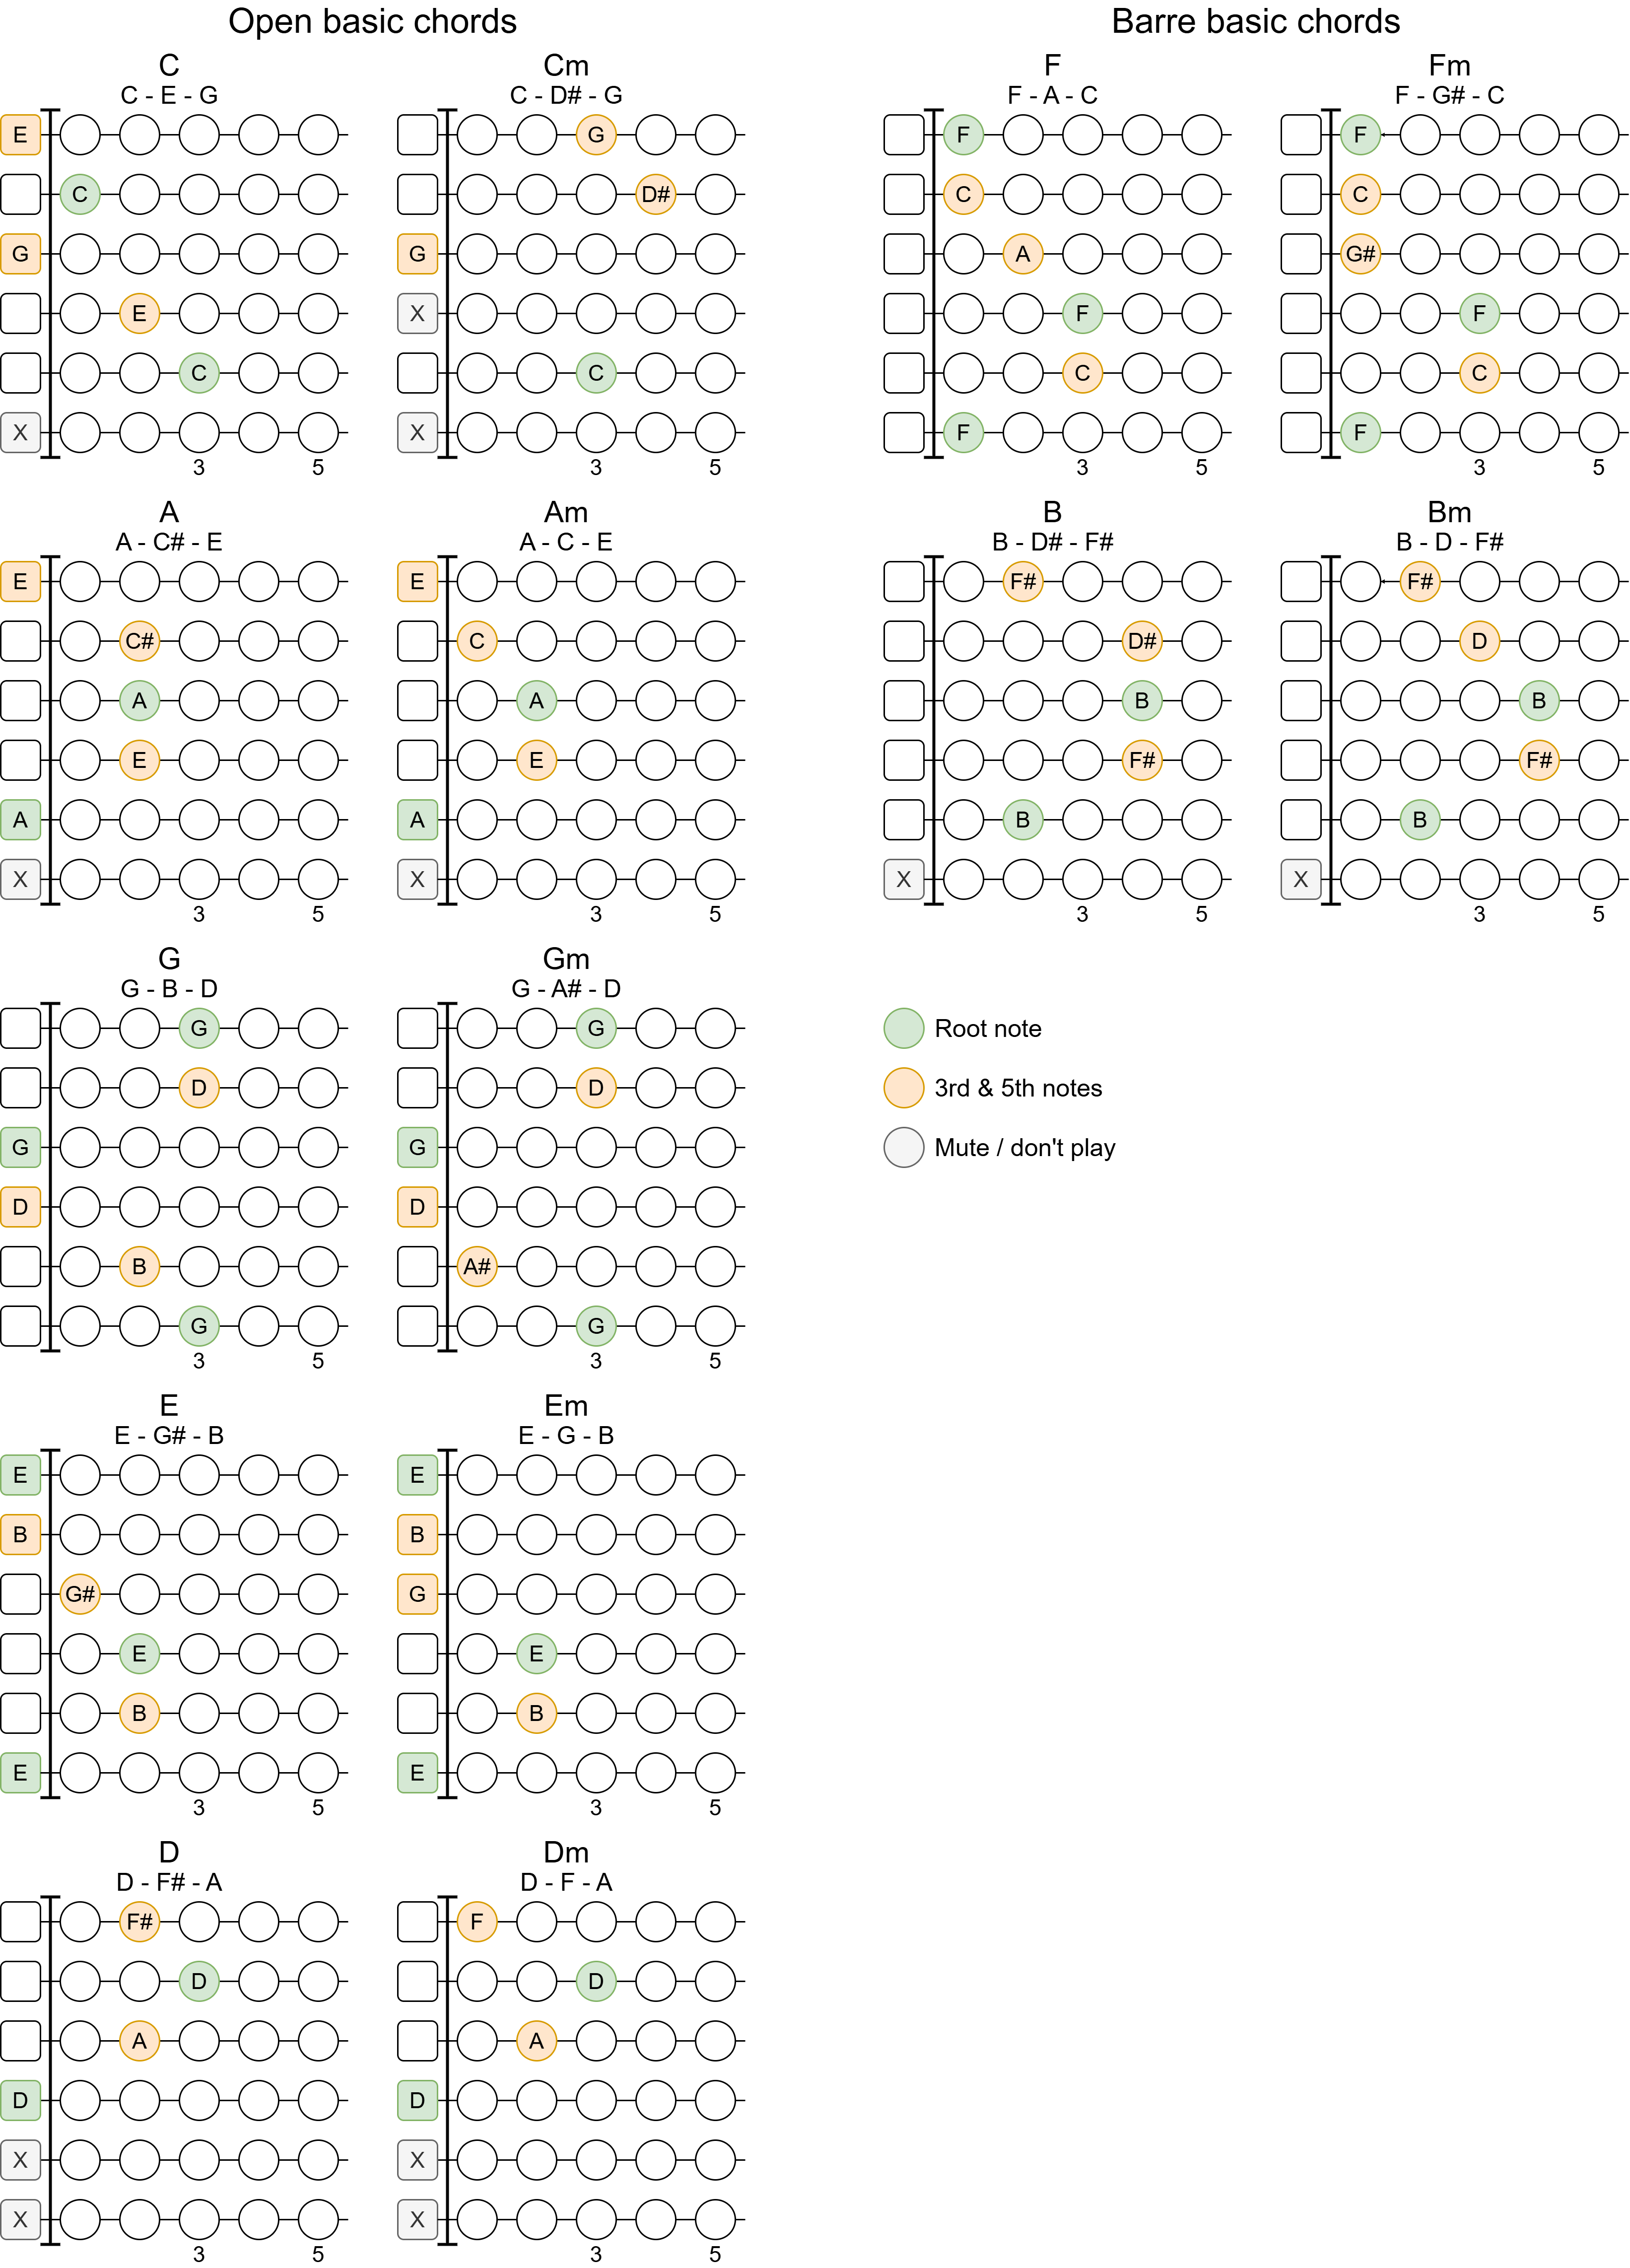
\includegraphics[height=0.8\textheight]{../../Images/GuitarBasicChords.png}
	\caption{Major and minor chords}
	\label{fig:guitar_major_minor_chords}
\end{figure}

\clearpage

Lets play some chords. The theme song of the Adventure Time series is a good start (\autoref{fig:guitar_adventure_time}). The notes on the staff here are replaced by rhythm notation. The duration of the note shapes is still the same. But now it only indicates the strumming rhythm.

The small symbol above the staff that looks like a square with an open bottom means a downstroke. This means that you play the chord by moving your hand/pick downwards through the string(s). The symbol above the staff that looks like a "V" is an upstroke. This means that you move your hand/pick upwards through the string(s).

\begin{figure}[h]
	\centering
	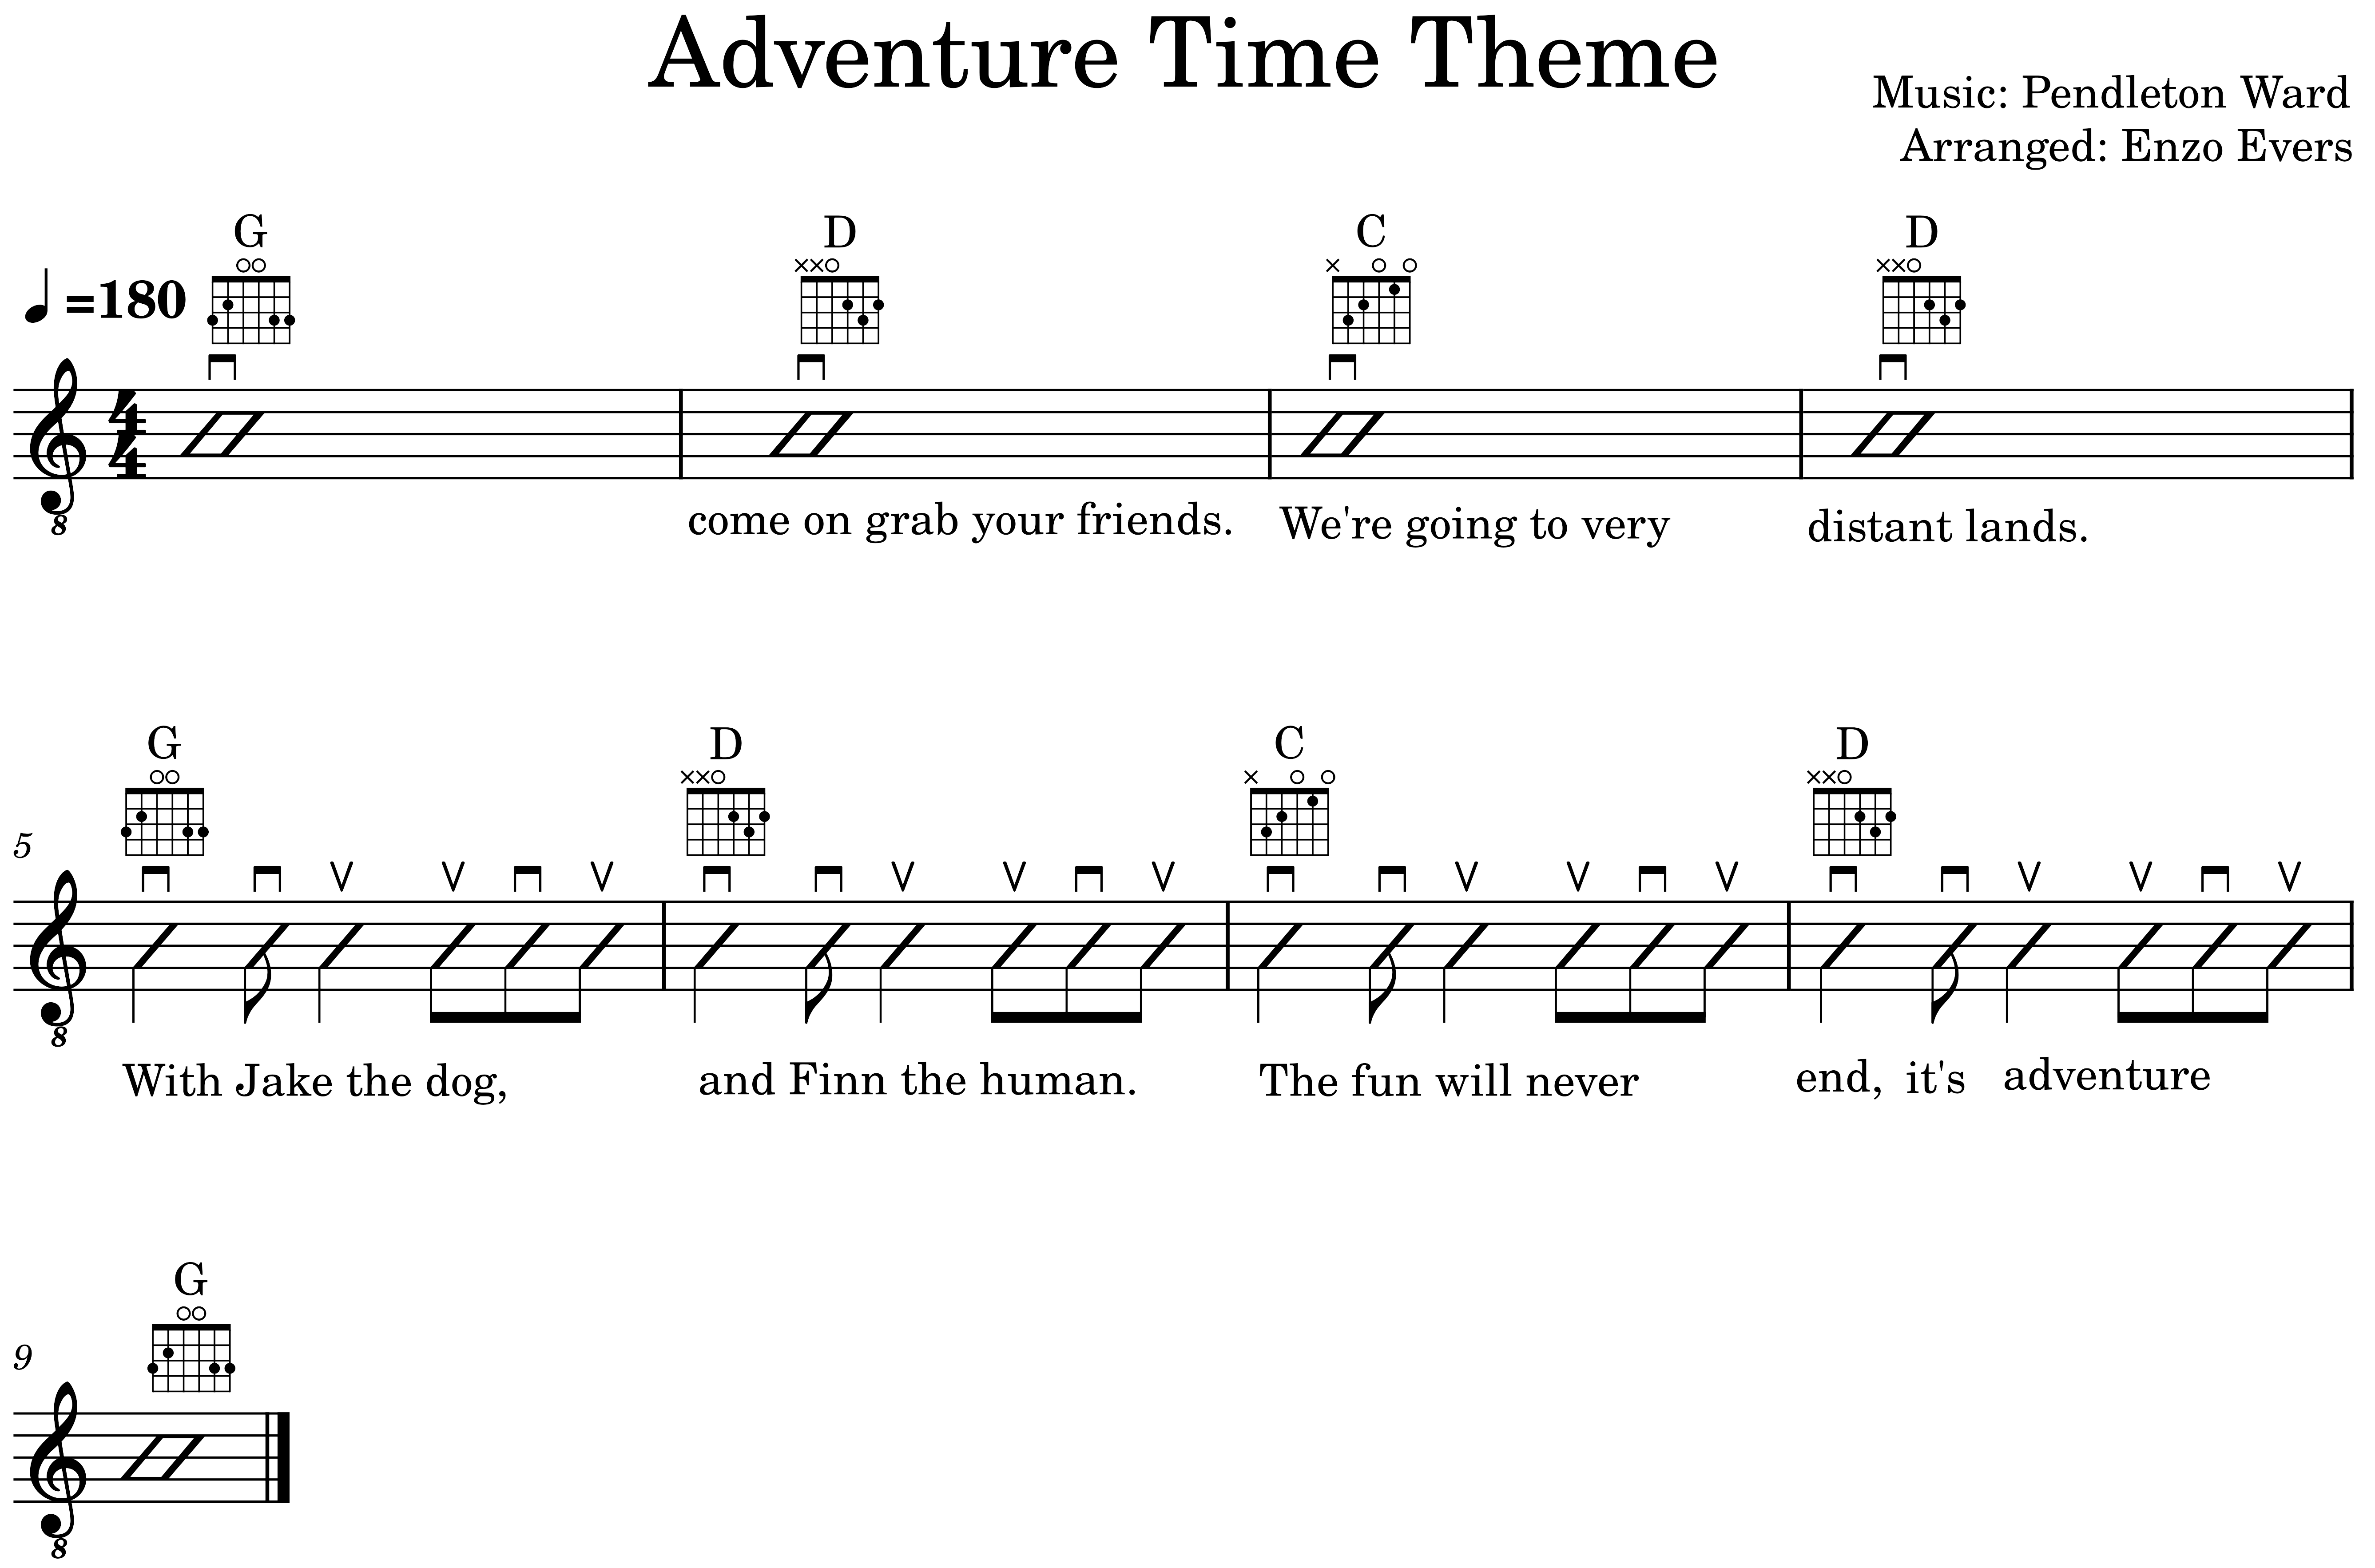
\includegraphics[width=\textwidth]{../../MuseScore/Guitar/GuitarAdventureTimeTheme.png}
	\caption{Adventure Time Theme Song}
	\label{fig:guitar_adventure_time}
\end{figure}

\newpage

In the song "Knockin' On Heaven's Door" By Bob Dylan, the same chords are used as in the Adventure Time theme, plus one extra chord. The \textbf{Am}.

\begin{song}[verse/numbered, remember-chords, align-chords=l]{title={Knockin' On Heaven's Door - Bob Dylan}, music={Bob Dylan}}
	\begin{intro}	
		^{G}   ^{D}      ^{Am}     ^{G}Oo ^{D}oo-oo ^{C}oo \\
		^{G}Oo ^{D}oo-oo ^{Am}oo   ^{G}Oo ^{D}oo-oo ^{C}oo \\
	\end{intro}
	\begin{verse}
		^{G}Mama, take this ^{D}badge off of me ^{Am} \\
		^{G}I can’t ^{D}use it anymore ^{C} \\
		^{G}It’s gettin’ ^{D}dark, too dark for me to see ^{Am} \\
		^{G}I feel like I’m ^{D}knockin’ on heaven’s door ^{C} \\
	\end{verse}
	\begin{chorus}
		^{G}Knock, knock, ^{D}knockin’ on heaven’s ^{Am}door \\
		^{G}Knock, knock, ^{D}knockin’ on heaven’s ^{C}door \\
		^{G}Knock, knock, ^{D}knockin’ on heaven’s ^{Am}door \\
		^{G}Knock, knock, ^{D}knockin’ on heaven’s ^{C}door \\
	\end{chorus}
	\begin{verse}
		^Mama, put my ^guns in the ground ^ {} \\
		^I can’t ^shoot them anymore ^ {} \\
		^That long black ^cloud is comin’ down ^ {} \\
		^I feel like I’m ^knockin’ on heaven’s door ^ {} \\
	\end{verse}
	\begin{chorus}
		^Knock, knock, ^knockin’ on heaven’s ^door \\
		^Knock, knock, ^knockin’ on heaven’s ^door \\
		^Knock, knock, ^knockin’ on heaven’s ^door \\
		^Knock, knock, ^knockin’ on heaven’s ^door \\
	\end{chorus}
\end{song}

\newpage

Another song to practice chord changes with is "Hey Ya!" from "Outkast". This only uses four chords, and the order of the chords is the same throughout the whole song.

To give a feel for the chords, the first part of the song is shown here. You can listen to the song and play these chords for the rest of the song.

\begin{song}[verse/numbered, align-chords=l]{title={Hey Ya! - Outkast}, music={Outkast}}
	\begin{intro}
		One, two, three, uh!
	\end{intro}
	\begin{verse}
		^{G}My baby don't ^{C}mess around \\
		Because she loves me so, and this ^{D}I know for ^{E}sure (Uh) \\
		^{G}But does she ^{C}really wanna \\
		But can't stand to see me walk ^{D}out the ^{E}door? (Ah) \\
	\end{verse}
\end{song}

\newpage

There are two (actually 4) more important shapes to learn. The closed barre shapes. These are shown in \autoref{fig:guitar_major_minor_chords} as the F, Fm, B, and Bm chords. For these chords you place your index finger over all the strings, and use the remaining fingers to press the remaining notes. Note that for the B chord you only have to place your index finger over the first 5 strings.

The song "Perfect" by Ed Sheeran is a good song to practice these shapes. This also shows the power of barre chords. The fact that they can be moved up and down the neck to make different chords.

The song uses 4 chords: A$\flat$, Fm, D$\flat$, and E$\flat$. Or if shown with sharps: G$\sharp$, Fm, C$\sharp$, and D$\sharp$.

Only the first verse is shown here to focus on the barre chords themselves. The barre chords to use are shown in \autoref{fig:guitar_barre_chords_perfect_ed_sheeran}. Note the numbers below the shapes. These are the fret numbers.


\begin{figure}[h]
	\centering
	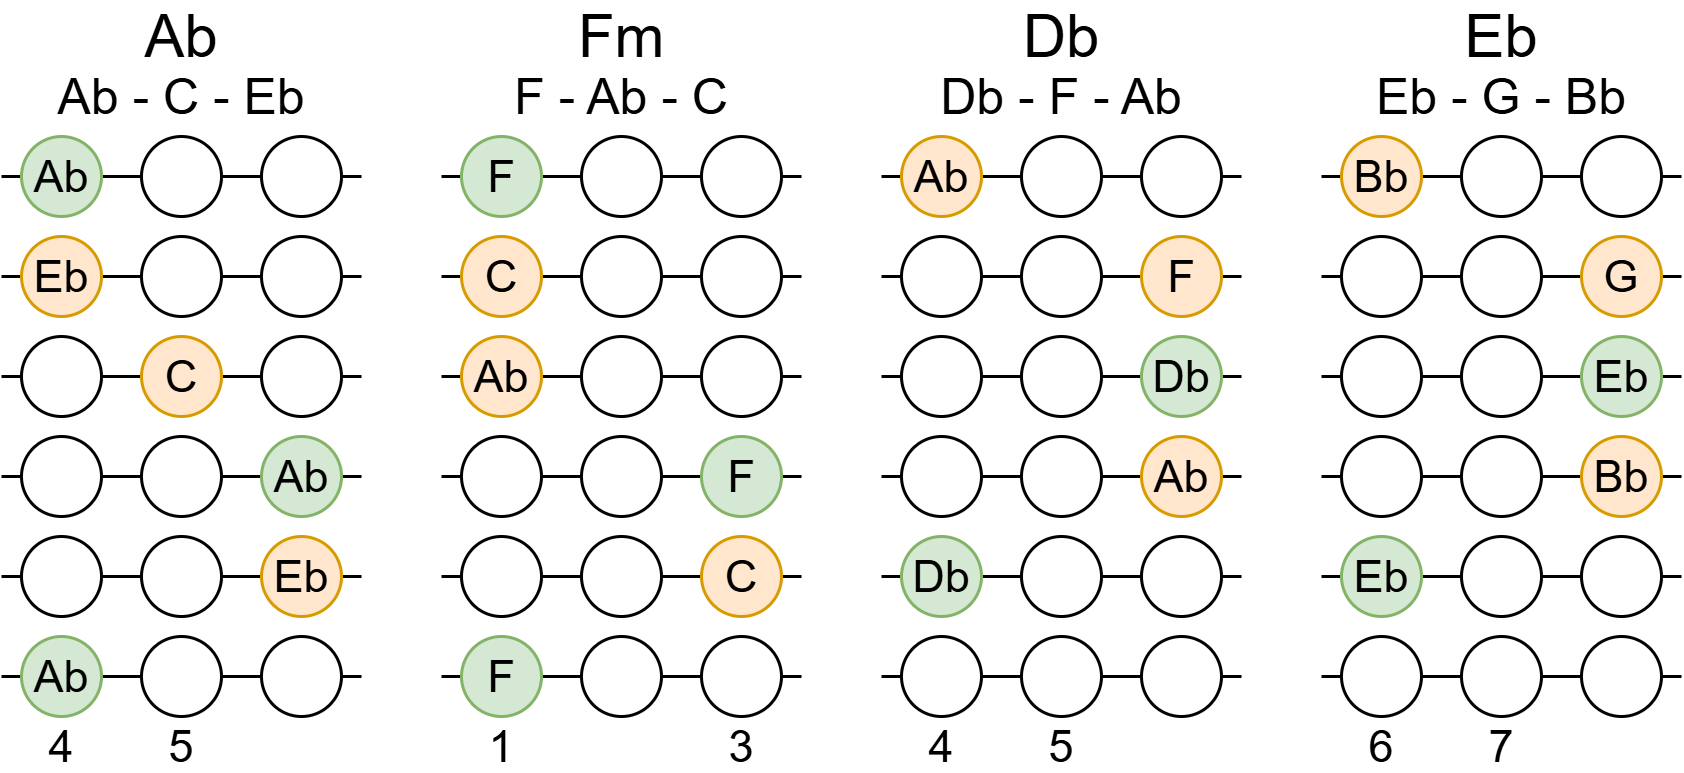
\includegraphics[width=0.8\textwidth]{../../Images/ChordsUsedInPerfectEdSheeran.png}
	\caption{Barre chords used in "Perfect - Ed Sheeran"}
	\label{fig:guitar_barre_chords_perfect_ed_sheeran}
\end{figure}


Note how the shapes are all very similar, but that the note on the lowest string indicates which chord name it is.

\infobox{It is not a rule that the note on the lowest string indicates the chord for all shapes. The combination of notes determine the chord. You will learn more about this later on.}

\begin{song}[verse/numbered, align-chords=l]{title={Perfect - Ed Sheeran}, music={Ed Sheeran}}
	\begin{verse}
		I found a ^{Ab}love for ^{Fm}me \\
		Oh, darling, just ^{Db}dive right in and follow my ^{Eb}lead \\
		Well, I found a ^{Ab}girl, beauti^{Fm}ful and sweet \\
		Oh, I never ^{Db}knew you were the someone waitin' for^{Eb}me \\
	\end{verse}
\end{song}

\subsection{Your turn}

We've played all kind of different chords now. It's up to you to see which song you want to play, look up the chords on the internet, and practice the chord transitions. Feel free to play the chords in different ways/shapes. Each option gives a different sound, or maybe one option is easier to play within the transition than another. Just experiment!